\documentclass{article}

\usepackage{graphicx}
\usepackage{hyperref}

\begin{document}

	\section*{Programming-Challenge Weatherdata by Maike Latsch}
	
	This program takes a csv file with weather or football data and finds the data with the smallest spread of two columns.
	
	In \autoref{fig:classDiagram} you can find a sketch of the class diagram. The system consists of two subsystems. The upper subsystem takes care of the analysis logic, while the lower one reads the CSV files.

	\begin{figure}[h]
		\centering      
		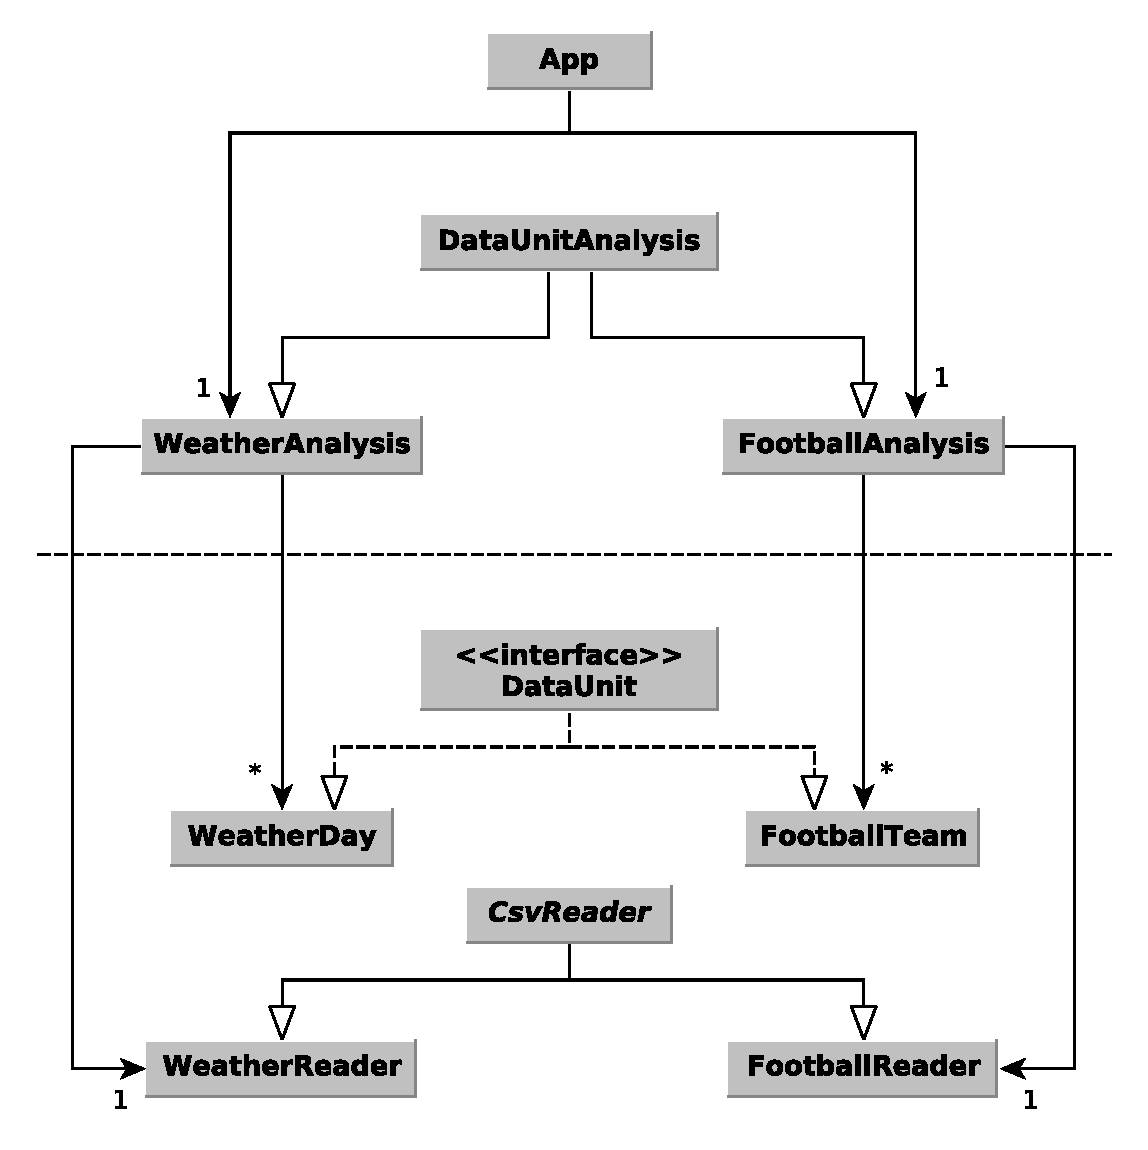
\includegraphics[width=10cm]{graphics/challenge-weatherdata.pdf}      
		\caption{class diagram sketch}
		\label{fig:classDiagram}
	\end{figure}
	
	\subsection*{Analysis}
	
	The main class of the analysis subsystem is DataUnitAnalysis. All other classes of this packages inherit from it. It has methods to perform mathematical analysis of DataUnits.
	
	The WeatherAnalysis inherits from DataUnitAnalysis and is specialized for weather data.
	
	The FootballAnalysis inherits from DataUnitAnalysis and is specialized for football data.
	
	\subsection*{Reader}
	
	The reader subsystem contains the csv readers and the DataUnits, which are used to communicate with the analysis.
	
	CsvReader is an abstract class, where the WeatherReader and the FootballReader are inheriting from. The CsvReader contains methods to parse in general csv data, while the WeatherReader is specialized for weather data and the FootballReader is specialized for football data. 
	
	All CsvReader communicate with the analysis subsystem using classes, which implement the interface DataUnit. The weather reader uses the WeatherDay and the FootballReader uses FootballTeam.
	
\end{document}